
\documentclass[handout, xcolor=dvipsnames]{beamer}

\usepackage{animate}
\usepackage{url}
\mode<presentation> {

\usetheme{Berlin}
\usetheme{Warsaw}

\setbeamertemplate{itemize items}[ball] % if you want a ball
\setbeamertemplate{itemize subitem}[circle] % if you wnat a circle
\setbeamertemplate{itemize subsubitem}[triangle] % if you want a triangle

\setbeamertemplate{blocks}[rounded][shadow=true]
\setbeamertemplate{navigation symbols}{}
\setbeamertemplate{mini frames}[square]
\setbeamersize{text margin left=6mm, text margin right=4mm}
\setbeamercolor{button}{bg = white, fg = blue}


\defbeamertemplate*{footline}{my theme}
 {
  \leavevmode%
  \hbox{%
  \begin{beamercolorbox}[wd=.35\paperwidth,ht=2.25ex,dp=1ex,center]{author in head/foot}%
    \usebeamerfont{author in head/foot}\insertshortauthor%~~(\insertshortinstitute USU)
  \end{beamercolorbox}%
  \begin{beamercolorbox}[wd=.65\paperwidth,ht=2.25ex,dp=1ex,center]{title in head/foot}%
    \usebeamerfont{title in head/foot}\insertshorttitle
  \end{beamercolorbox}%
  \begin{beamercolorbox}[wd=.1\paperwidth,ht=2.25ex,dp=1ex,right]{date in head/foot}%
     %\usebeamerfont{date in head/foot}\insertshortdate{}\hspace*{2em}
    %\insertframenumber{}\hspace*{2ex} 
  \end{beamercolorbox}}%
  \vskip0pt%
}

 % or ...

  \setbeamercovered{transparent}
  % or whatever (possibly just delete it)
}


\usetheme{Darmstadt}
\usefonttheme[onlylarge]{structurebold}
\setbeamerfont*{frametitle}{size=\normalsize,series=\bfseries}
\setbeamertemplate{navigation symbols}{}

\usepackage[english]{babel}
\usepackage{multirow}
\usepackage[latin1]{inputenc}
\usepackage{times}
\usepackage[T1]{fontenc}
\usepackage{graphicx}
\usepackage{natbib} %citep and citet
\usepackage{color}

%%% for references
\renewcommand{\bibsection}{\subsubsection*{\bibname}} % to avoid References creates new section/subsection in header
\bibpunct[:]{(}{)}{;}{a}{}{,}




\begin{document}

% here you define the information that will be displayed in the title/cover page

\title[\hspace*{0.5cm} 2025, Logan, Utah, United States of America
	   \hspace*{80pt}\hfill \insertframenumber\hspace*{0.5cm}]
       {Call of the Data Analysis 2025:  \\ 
       Viewing Climate Change across the Globe}


\author[\hspace*{0cm}\hfill \hspace*{0.25cm}]
		{Adelynn Shirts, Spencer DenBleyker, & Zayne Maughan} \\[-2.2cm]

}

\date{April 18, 2025}


% here you build the title page
\frame{
  \titlepage
}


% outline 
%\AtBeginSection[]
%{
%  \begin{frame}<beamer>{outline}
%    \frametitle{Outline}
%    \small
%    \tableofcontents[currentsection]%,hideothersubsections]
%    \normalsize
%  \end{frame}
%}


% If you wish to uncover everything in a step-wise fashion, uncomment
% the following command:

%\beamerdefaultoverlayspecification{<+->}


%%%%%%%%%%%%%%%%%%%%%%%%%
%%%   Outline           %
%%%%%%%%%%%%%%%%%%%%%%%%%

\begin{frame} 
\frametitle{Outline}
  \tableofcontents
  % You might wish to add the option [pausesections]
\end{frame}

%\newcounter{finalframe}

%%%%%%%%%%%%%%%%%%%%%%%%%
%\section{Introduction}  
%%%%%%%%%%%%%%%%%%%%%%%%%


%%%%%%%%%%%%%%%%%%%%%%%%%
\section{Overview}  
%%%%%%%%%%%%%%%%%%%%%%%%%

\subsection{}
\begin{frame}
	\frametitle{Primary Research Question}
	\begin{itemize}
    	\item The center of the competition is centered on the analysis of \textbf{climate change and related events, exploring their impacts.} 
    	\item Main Question: How has climate change effected the world over the last 30 years? 
    	\item Breaking this down into four main categories: 
            \begin{itemize}
                \item Annual Surface Temperature
                \item Mean Sea Level Change
                \item Climate Related Disasters
                \item Forest and Carbon Levels
            \end{itemize}
    \end{itemize}
\end{frame}


\subsection{}
\begin{frame}
	\frametitle{Data}
	\begin{itemize}
%	\item Several preliminary test participants (2 presented here)
    	\item Annual Surface Temperature
            \begin{itemize}
                \item From 1961 to 2023 over different countries and regions
            \end{itemize}
    	\item Mean Sea Level Change
            \begin{itemize}
                \item 1992 - 2025 over various regions
            \end{itemize}
    	\item Climate Related Disasters
            \begin{itemize}
                \item 1980 - 2024 over a plethora of countries and regions
            \end{itemize}
            \item Forest and Carbon Levels
            \begin{itemize}
                \item 1992 - 2022 focused on forested areas and carbon footprint
                of countries around the globe
            \end{itemize}
    \end{itemize}
\end{frame}


\subsection{}
\begin{frame}
	\frametitle{Key Questions}
	\begin{itemize}
    	\item How has the surface temperature increased over the past 60 years?
    	\item How has sea level changed over the last 30 years?
            \item Have climate related disasters increased over the last 40 years? 
                \subitem Are there any regions that seem more disposed to these disasters?
            \item Has deforestation played a large role into these other categories?
    \end{itemize}
\end{frame}

%%%%%%%%%%%%%%%%%%%%%%%%%
\section{Data, Code, and Packages}  
%%%%%%%%%%%%%%%%%%%%%%%%%
\subsection{}
\begin{frame}
	\frametitle{Data}
	\begin{itemize}
    	\item All data was exported from the IMF's different websites regarding their climate data. Three websites in total which will be found at the references slide. 
    	\item The Mean Sea Level Change and Annual Surface Temperature were found at the climate and weather page. 
    	\item The Climate Related Disasters was found on the Adaptation page or dashboard.
    	\item The forest and carbon levels data was found on the Mitigation page.
    \end{itemize}
\end{frame}

\subsection{}
\begin{frame}
	\frametitle{Packages Used}
	\begin{itemize}
    	\item Since the data could be exported as csv files there was no need to scrape it from the web.
    	\item However, various other packages were used in the manipulation and wrangling stage. These include the following: 
            \item readr 
            \begin{itemize}
                \item easy reading in of the data,
            \end{itemize}
            \item dplyr 
            \begin{itemize}
                \item data manipulation,
            \end{itemize}
            \item tidyr 
            \begin{itemize}
                \item ensures data is fit for tidyverse use,
            \end{itemize}
            \item forcats 
            \begin{itemize}
                \item focuses on factors.
            \end{itemize}
    	\item countrycode 
        \begin{itemize}
                \item a convenient way to convert different country codes for data manipulation
        \end{itemize}
    \end{itemize}
\end{frame}


\subsection{}
\begin{frame}
	\frametitle{Packages Used}
	\begin{itemize}
    	\item ggplot2
        \begin{itemize}
            \item A basic plotting library
        \end{itemize}
    	\item rnaturalearth
        \begin{itemize}
            \item A package that provides ease of use maps of the world
        \end{itemize}
    	\item sf
               \begin{itemize}
                   \item  spatial features for better maps
               \end{itemize} 
    	\item gganimate
            \begin{itemize}
                \item create animated graphics
            \end{itemize}
    	\item gifski 
            \begin{itemize} 
                \item allow for animated graphics to be saved in gif format
            \end{itemize}
                
    \end{itemize}
\end{frame}

%%%%%%%%%%%%%%%%%%%%%%%%%
\section{Annual Surface Temp}  
%%%%%%%%%%%%%%%%%%%%%%%%%


\subsection{}

\begin{frame}
	\frametitle{Global Average Temperature over time}
	\begin{center} 
		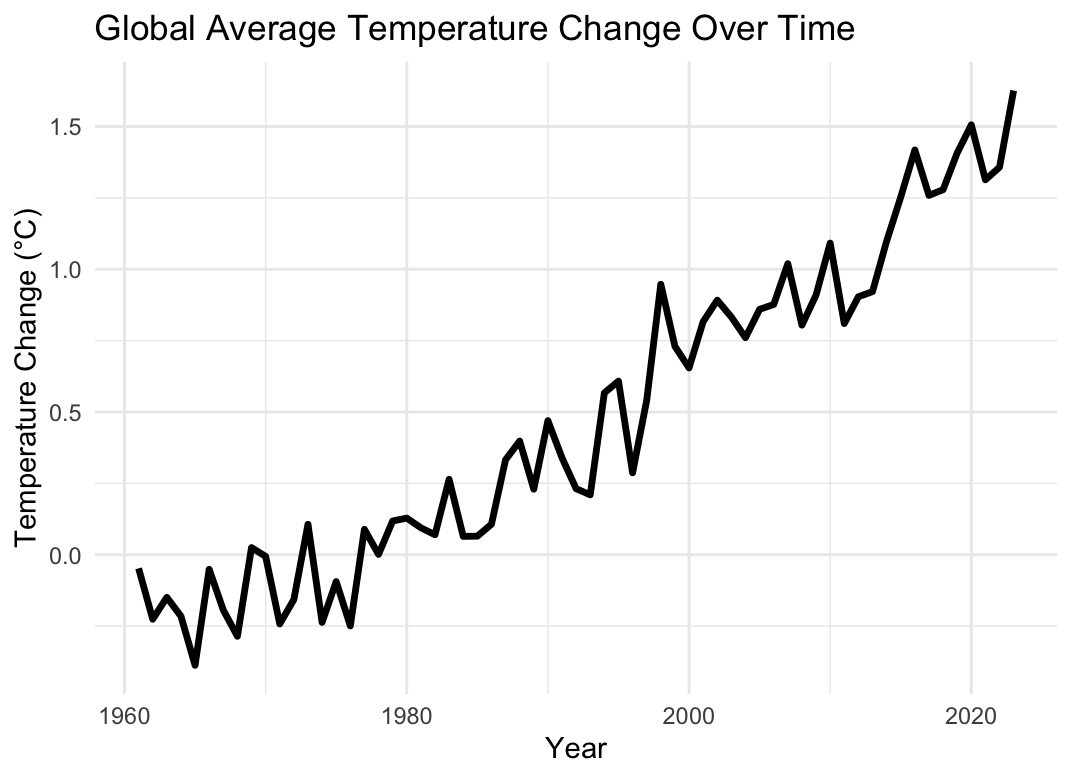
\includegraphics[width=5.5cm]{images/temperature_plots/Avg_temp_over_time.png} \hspace{1pt}
            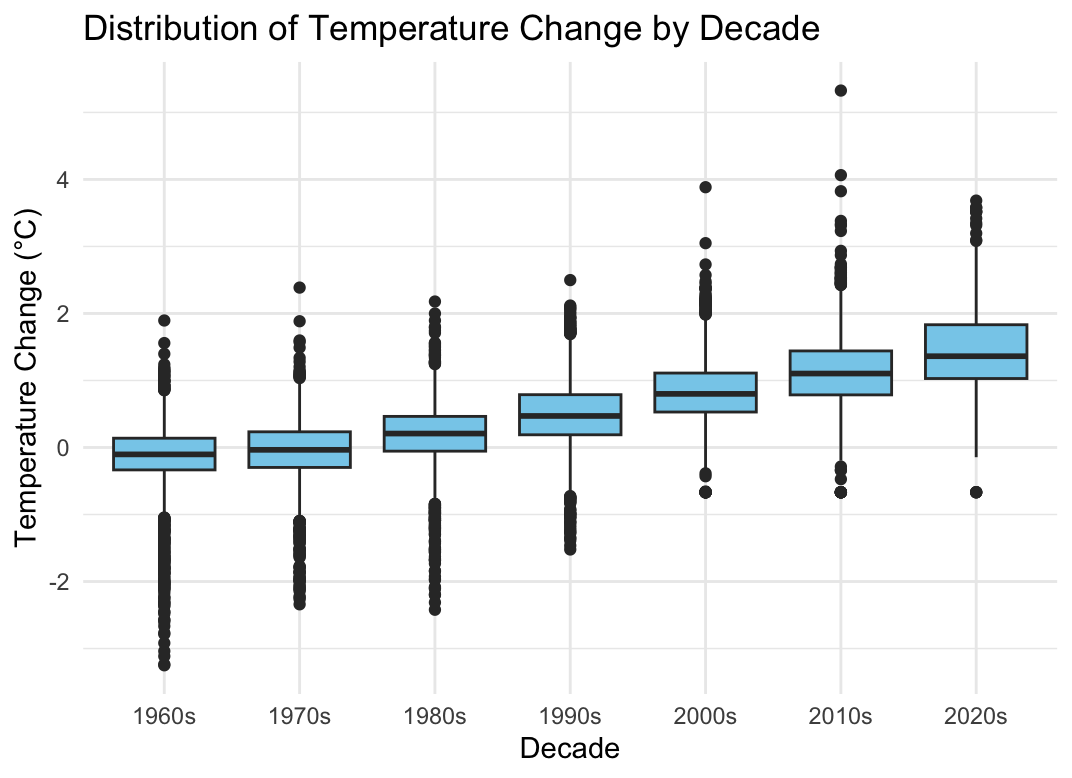
\includegraphics[width=5.5cm]{images/temperature_plots/boxplot_temp.png} \hspace{1pt}
	\end{center}
\end{frame}


\begin{frame}
	\frametitle{World Map of Average Temperature over the years}
	\begin{center} 
		\animategraphics[loop, autoplay, width=0.7\linewidth]{10}{images/temp_gif/frame_}{000}{080}
	\end{center}
\end{frame}

\begin{frame}
	\frametitle{Africa}
	\begin{center} 
		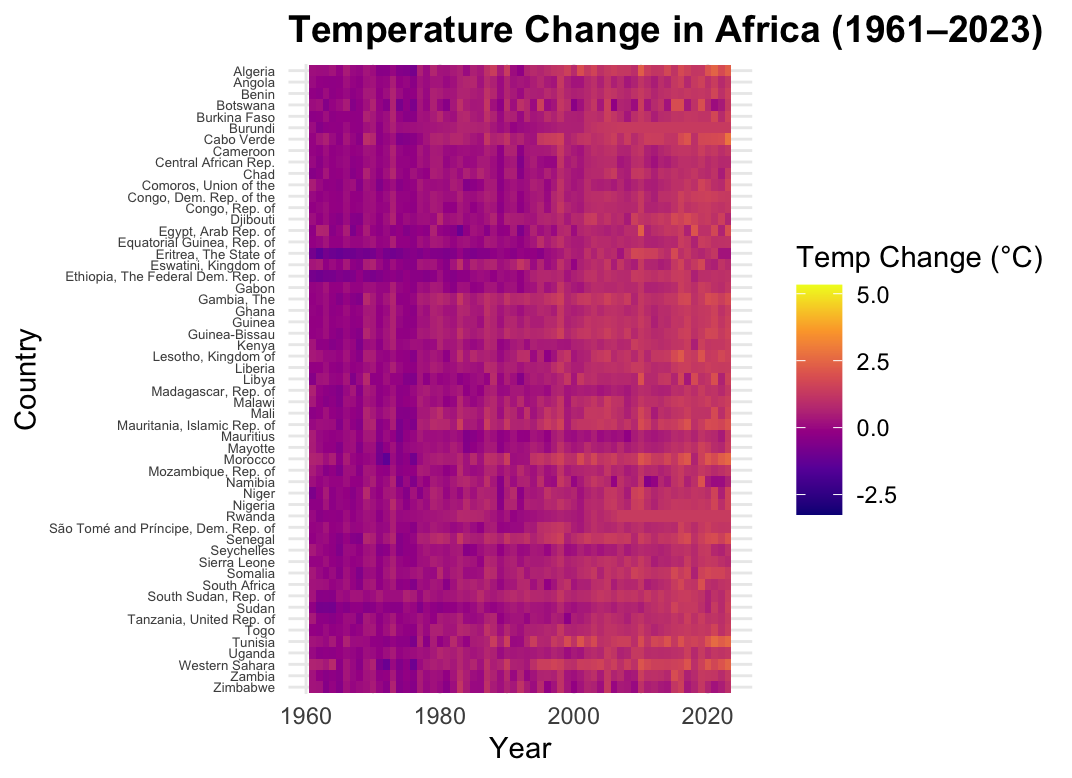
\includegraphics[width = 5.5cm]{images/heatmaps/Africa_heatmap_temp.png} \hspace{1pt}
            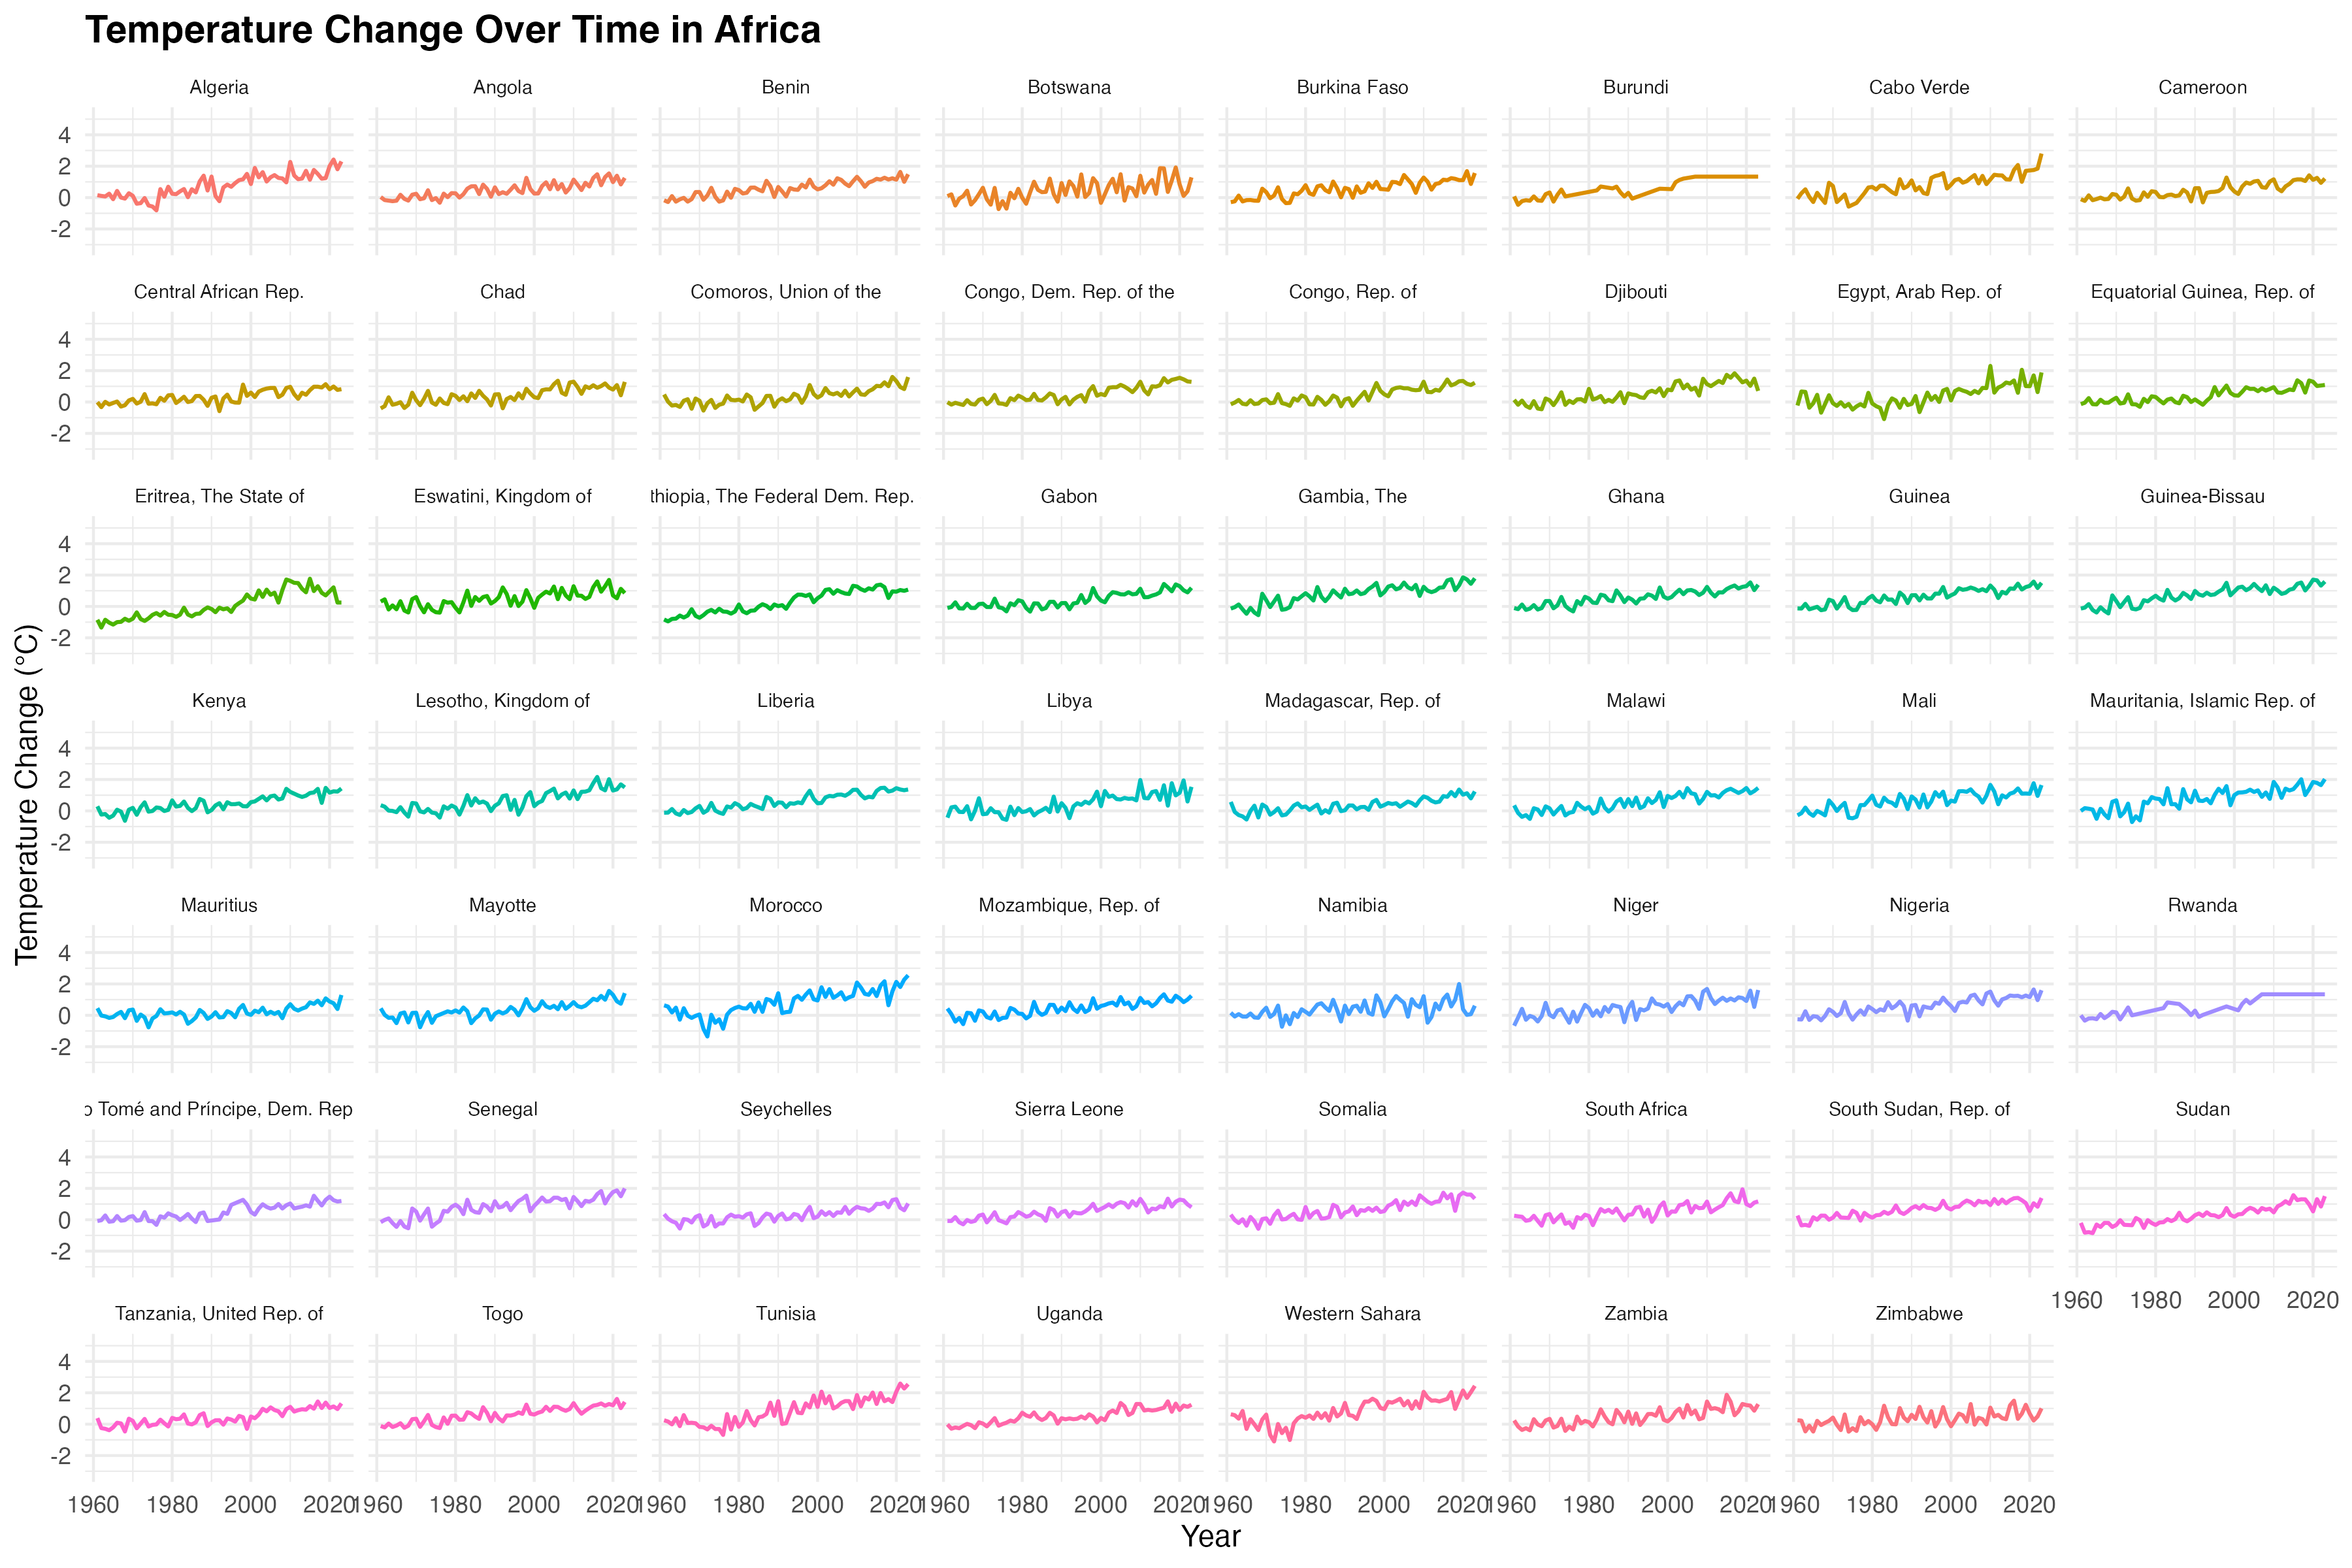
\includegraphics[width = 5.5cm]{images/temperature_plots/temperature_plot_Africa.png} \hspace{1pt}
	\end{center}
\end{frame}
    
\begin{frame}
	\frametitle{Americas}
	\begin{center} 
		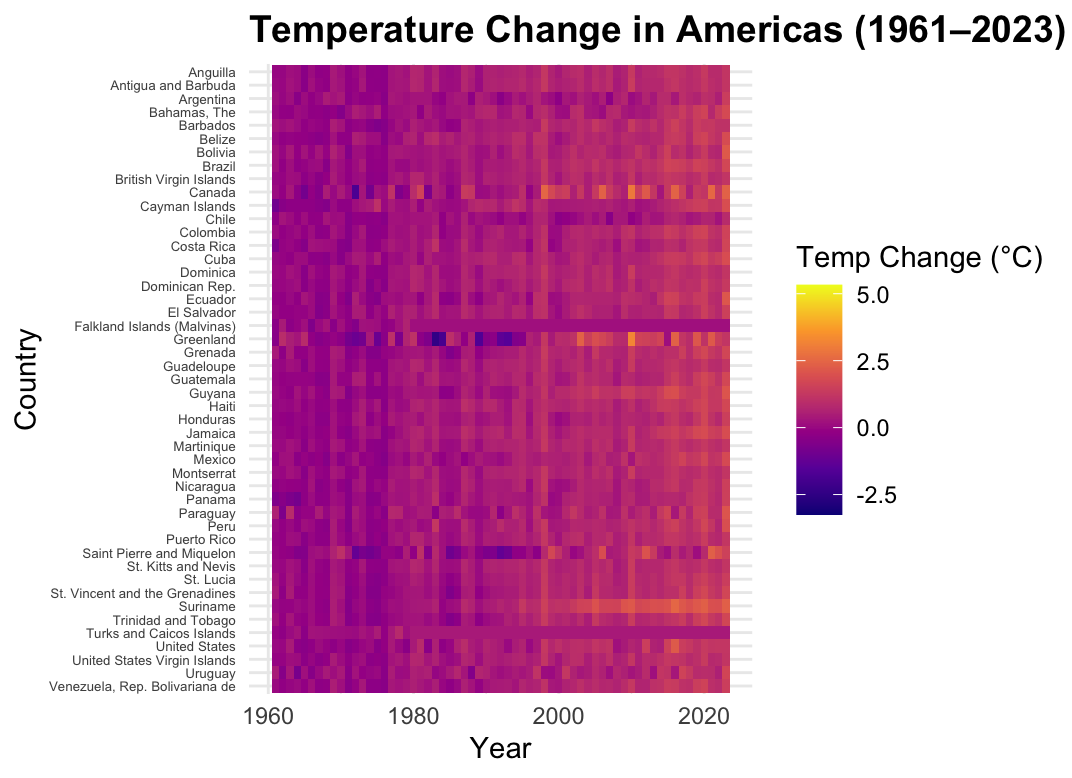
\includegraphics[width = 5.5cm]{images/heatmaps/America_heatmap_temp.png} \hspace{1pt}
            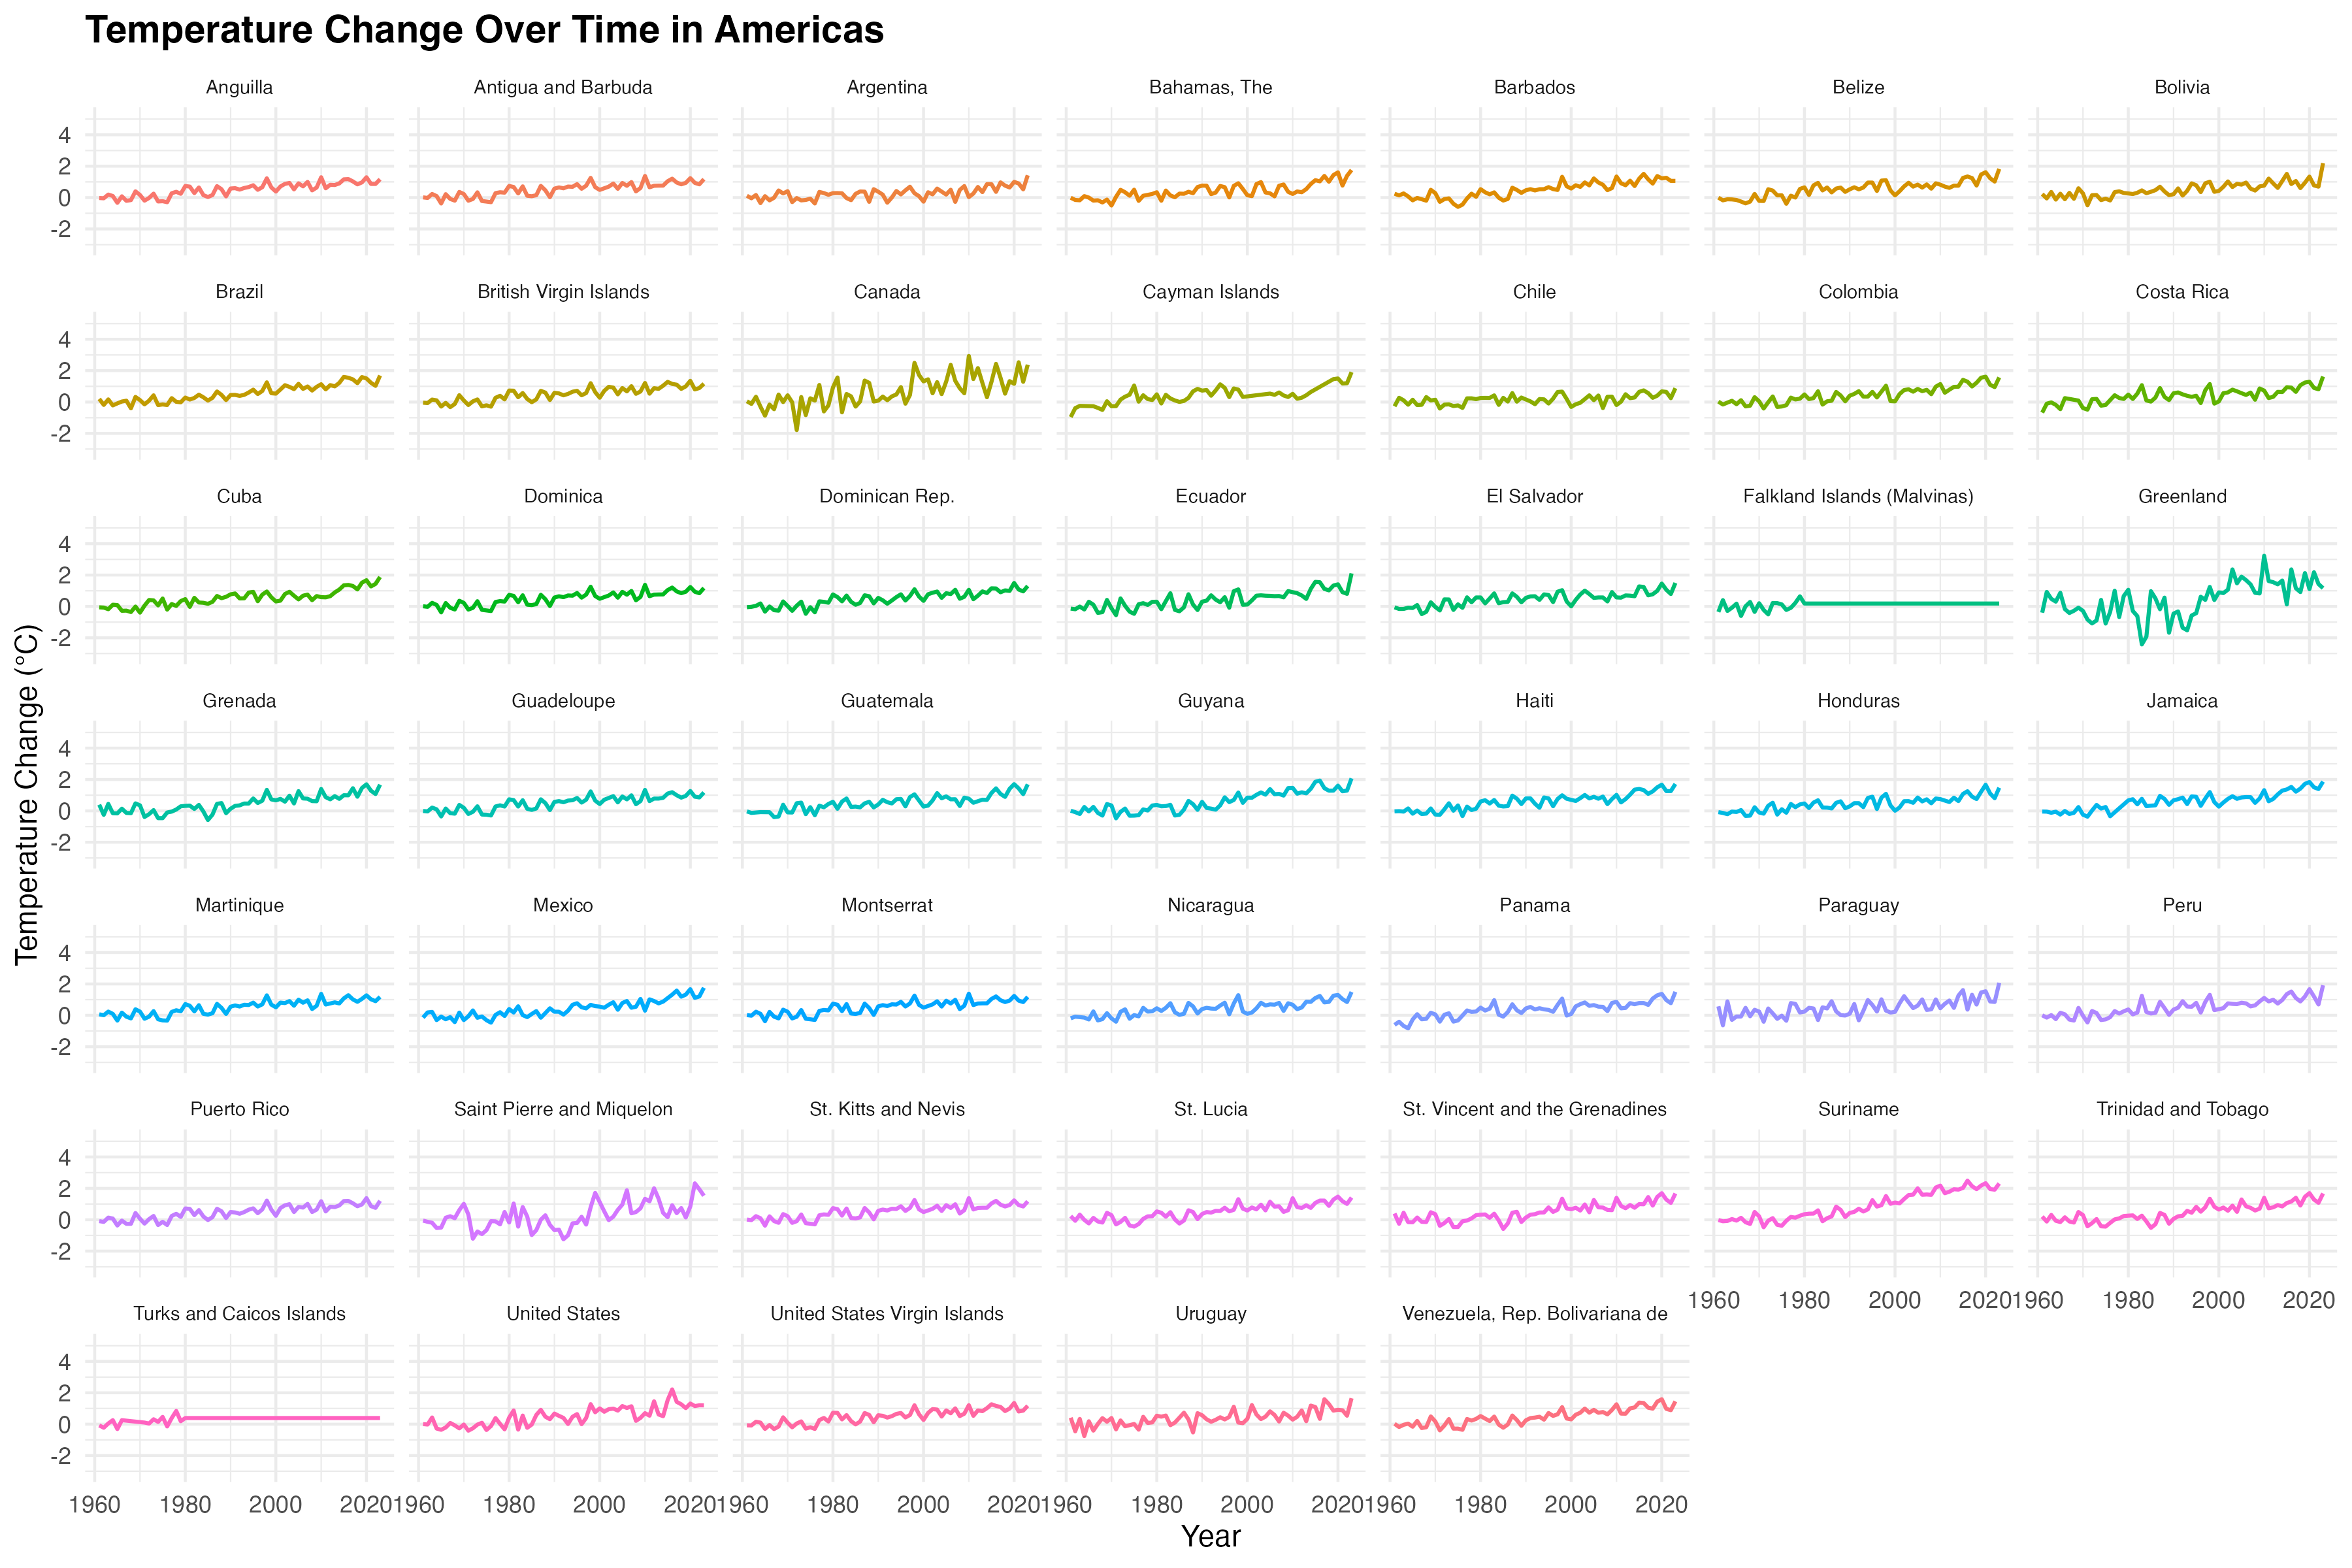
\includegraphics[width = 5.5cm]{images/temperature_plots/temperature_plot_Americas.png} \hspace{1pt}
	\end{center}
\end{frame}
    
\begin{frame}
	\frametitle{Asia}
	\begin{center} 
		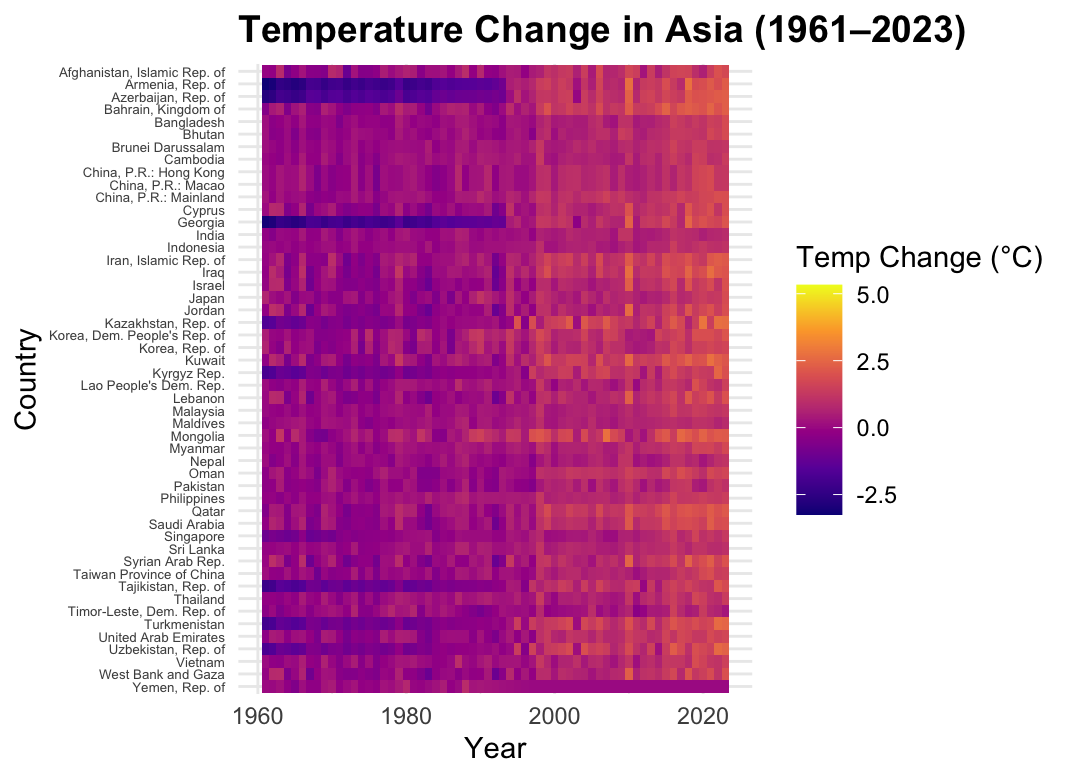
\includegraphics[width = 5.5cm]{images/heatmaps/Asia_heatmap_temp.png} \hspace{1pt}
            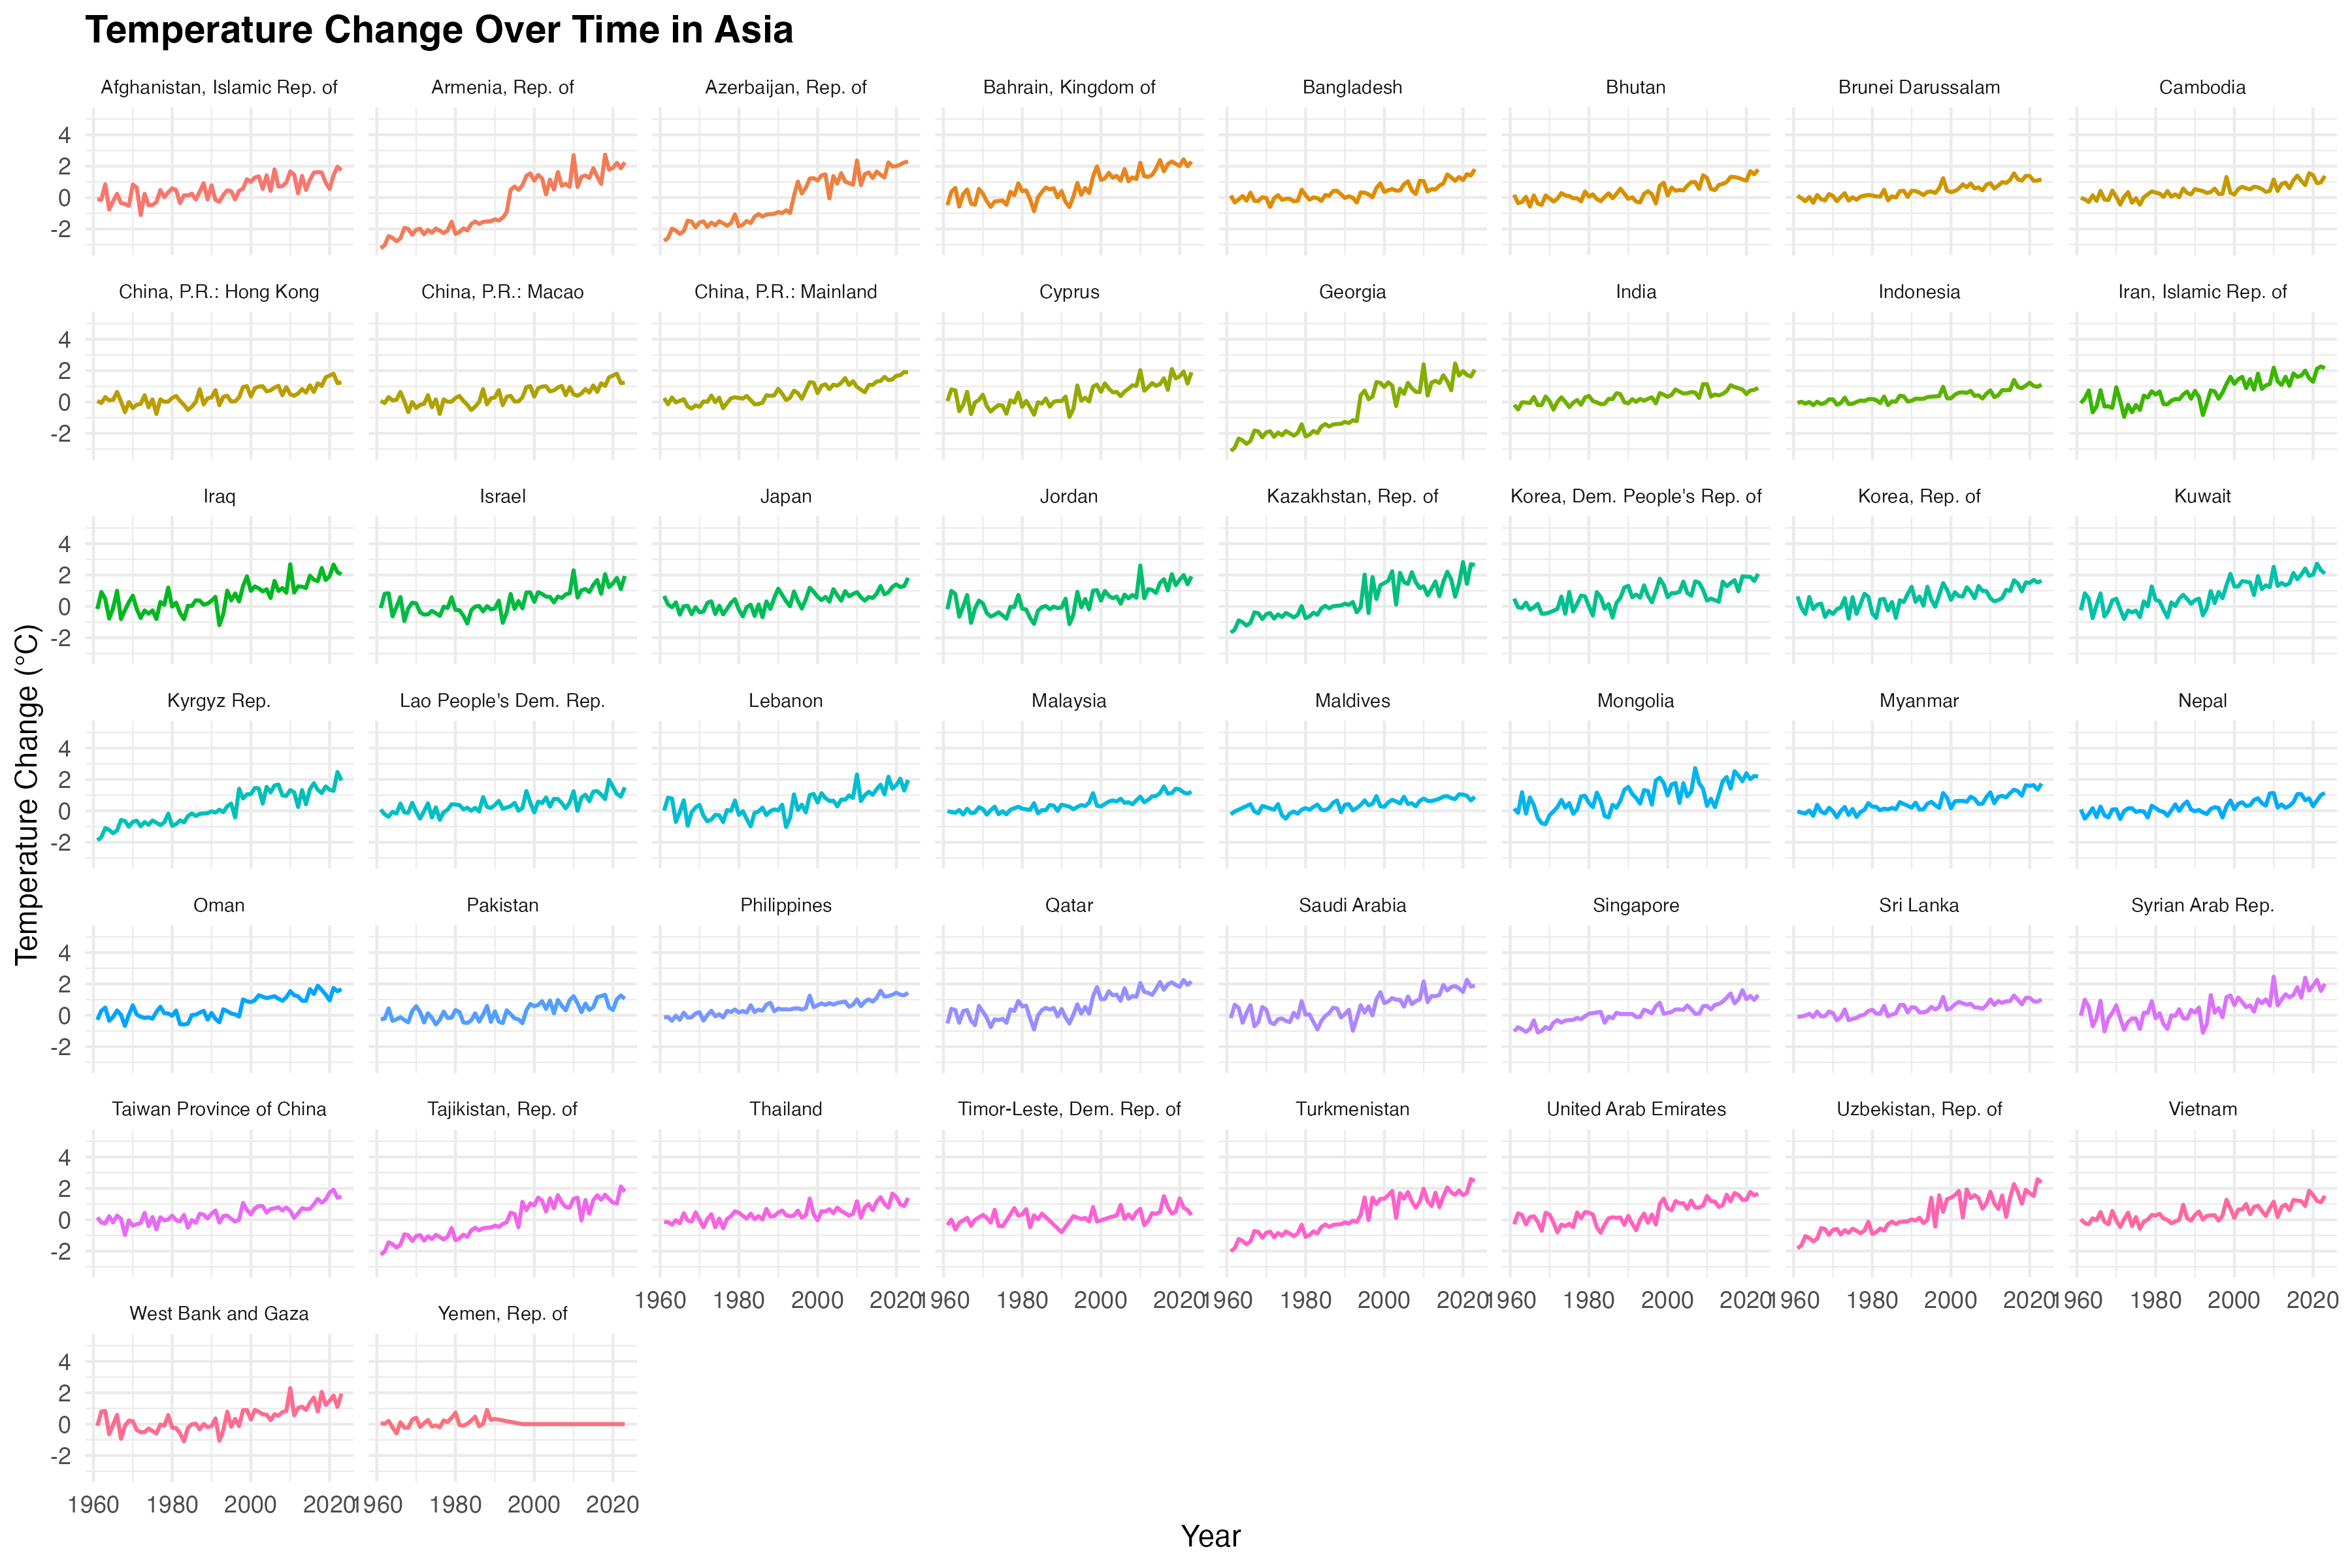
\includegraphics[width = 5.5cm]{images/temperature_plots/temperature_plot_Asia.png} \hspace{1pt}
	\end{center}
\end{frame}
    
\begin{frame}
	\frametitle{Europe}
	\begin{center} 
		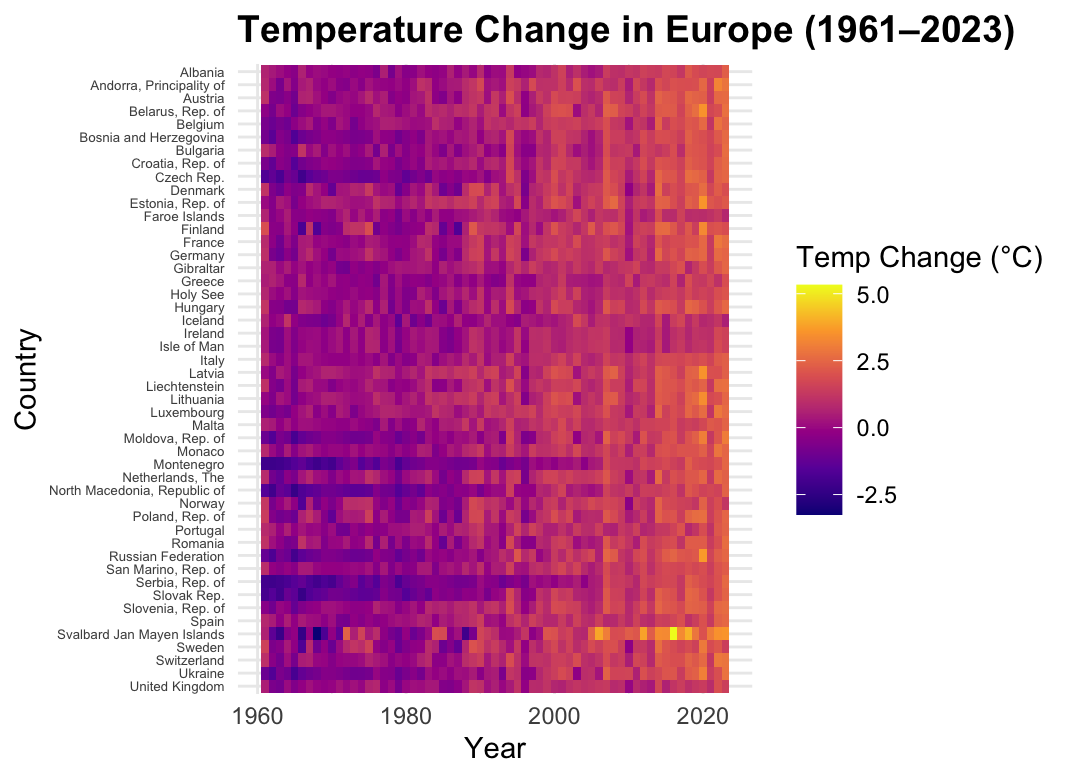
\includegraphics[width = 5.5cm]{images/heatmaps/Europe_heatmap_temp.png} \hspace{1pt}
            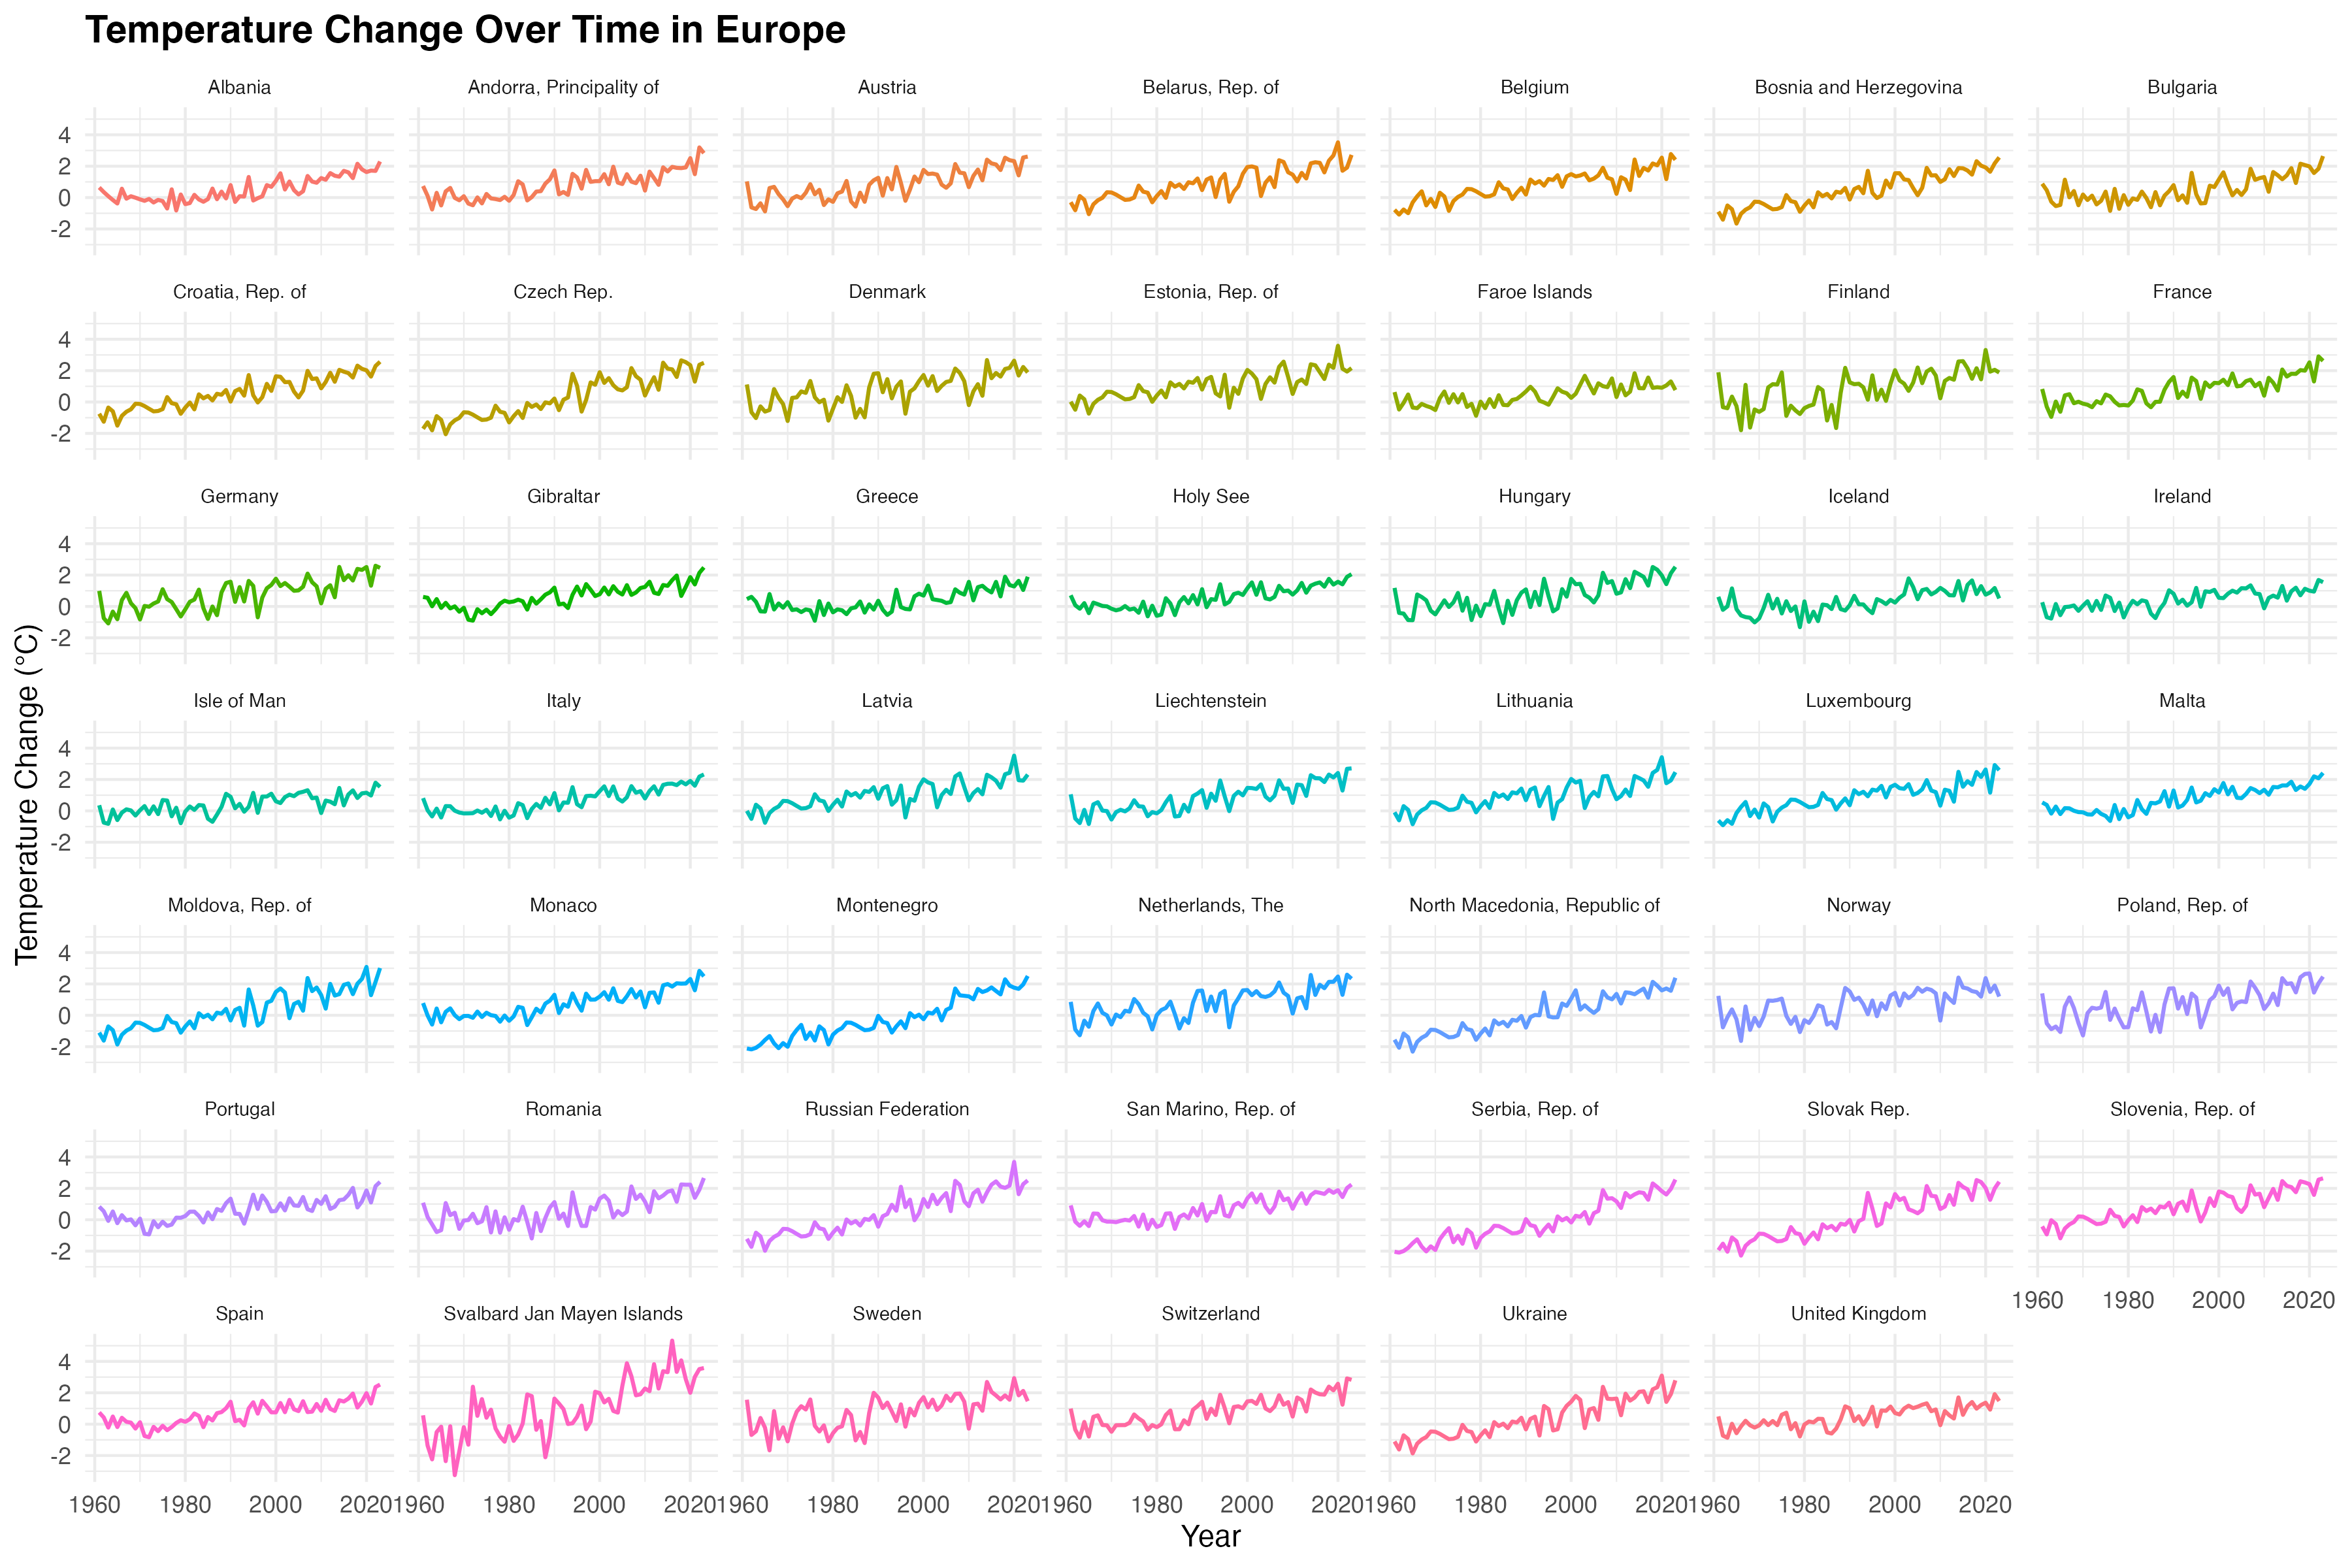
\includegraphics[width=5.5cm]{images/temperature_plots/temperature_plot_Europe.png} \hspace{1pt}
	\end{center}
\end{frame}
    
\begin{frame}
	\frametitle{Oceania}
	\begin{center} 
		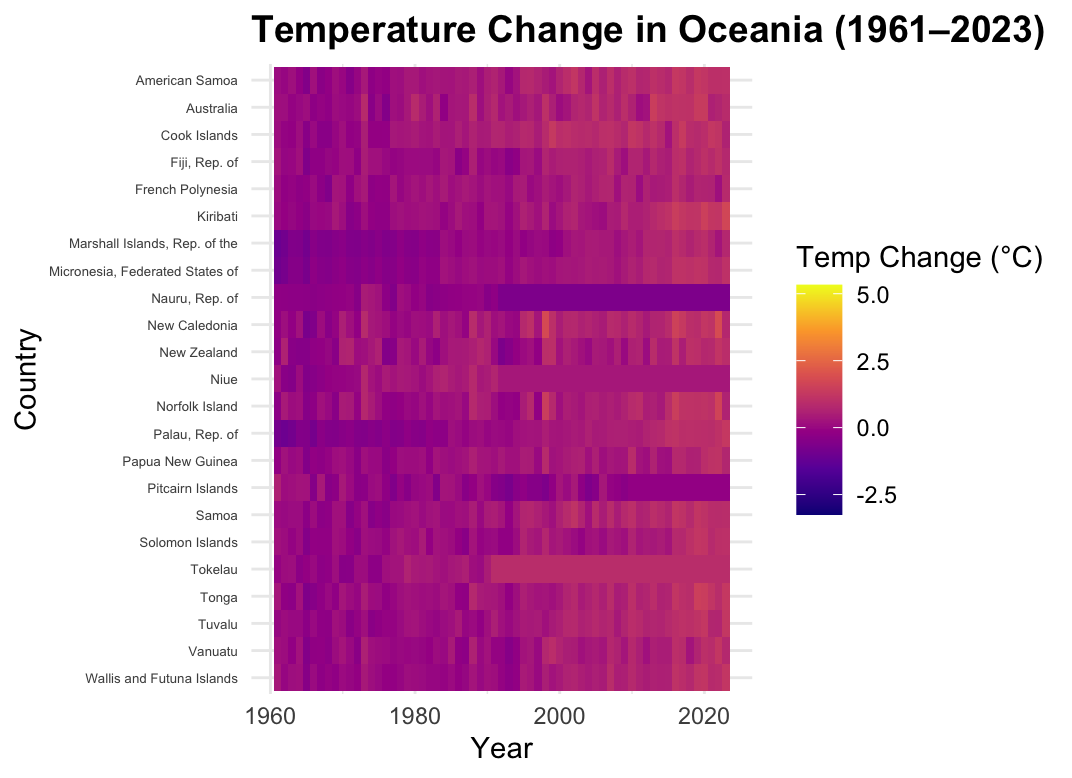
\includegraphics[width=5.5cm]{images/heatmaps/Oceania_heatmap_temp.png} \hspace{1pt}
            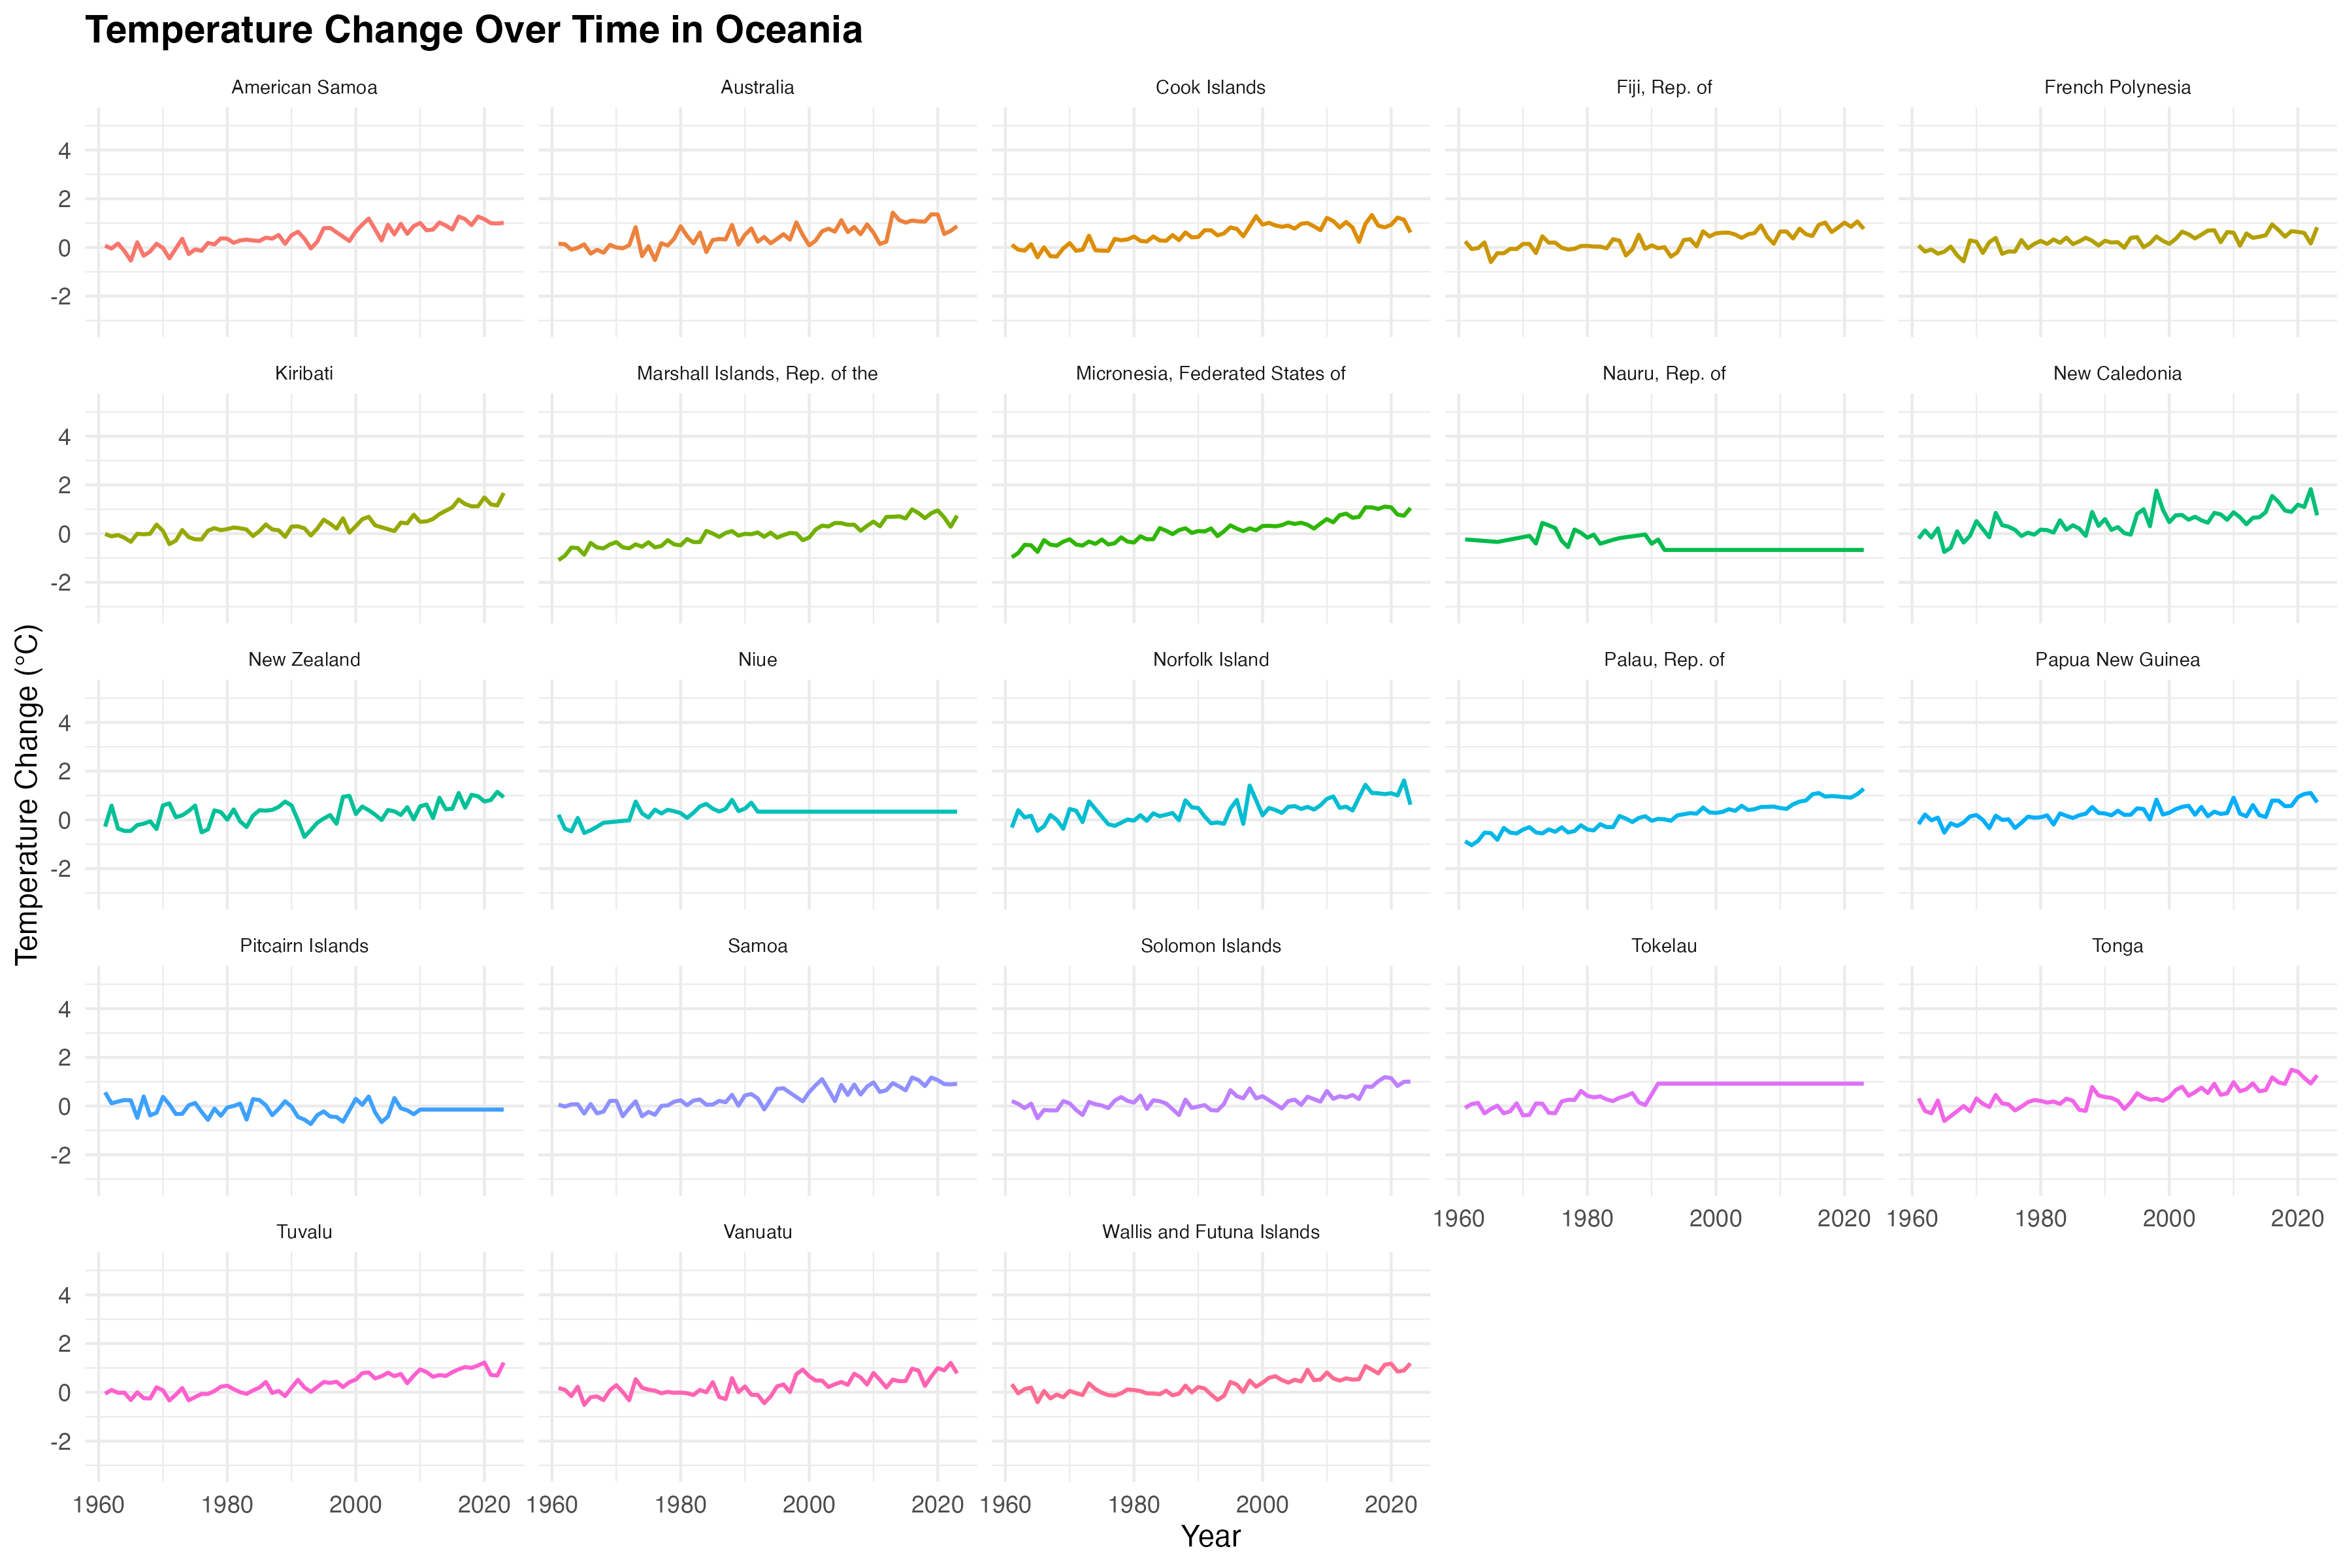
\includegraphics[width = 5.5cm]{images/temperature_plots/temperature_plot_Oceania.png} \hspace{1pt}
	\end{center}
\end{frame}
    
\subsection{}
\begin{frame}
	\frametitle{Remarks on Annual Surface Temp}
	\begin{itemize}
	\item It appears to have gotten warmer in every region and country but Oceania             had the smallest growth in Temperature. \\[1cm]
        \item This rise in temperatures will provide insight to the other categories and their relationship with the climate
    \end{itemize}
\end{frame}


%%%%%%%%%%%%%%%%%%%%%%%%%
\section{Climate Related Disaster}  
%%%%%%%%%%%%%%%%%%%%%%%%%


\subsection{}
\begin{frame}
	\frametitle{Disasters by region} % Posture 8
	\begin{center} 
		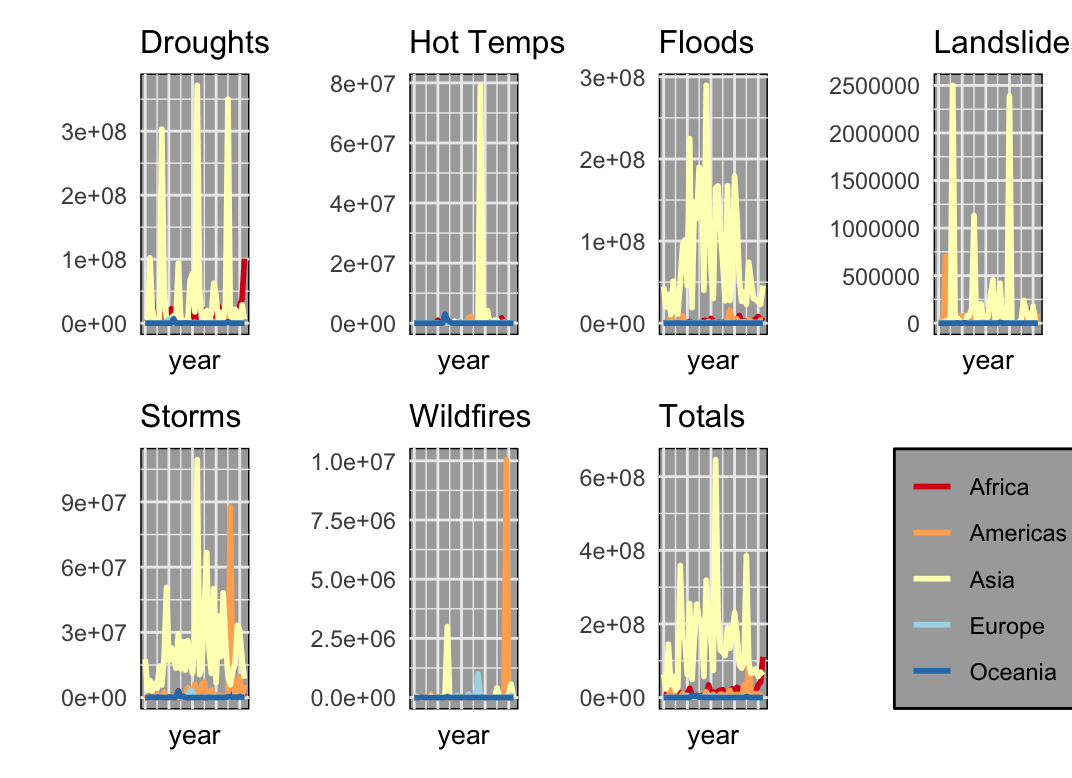
\includegraphics[width=5.5cm]{images/disaster/Disaster_area.png} \hspace{1pt}
		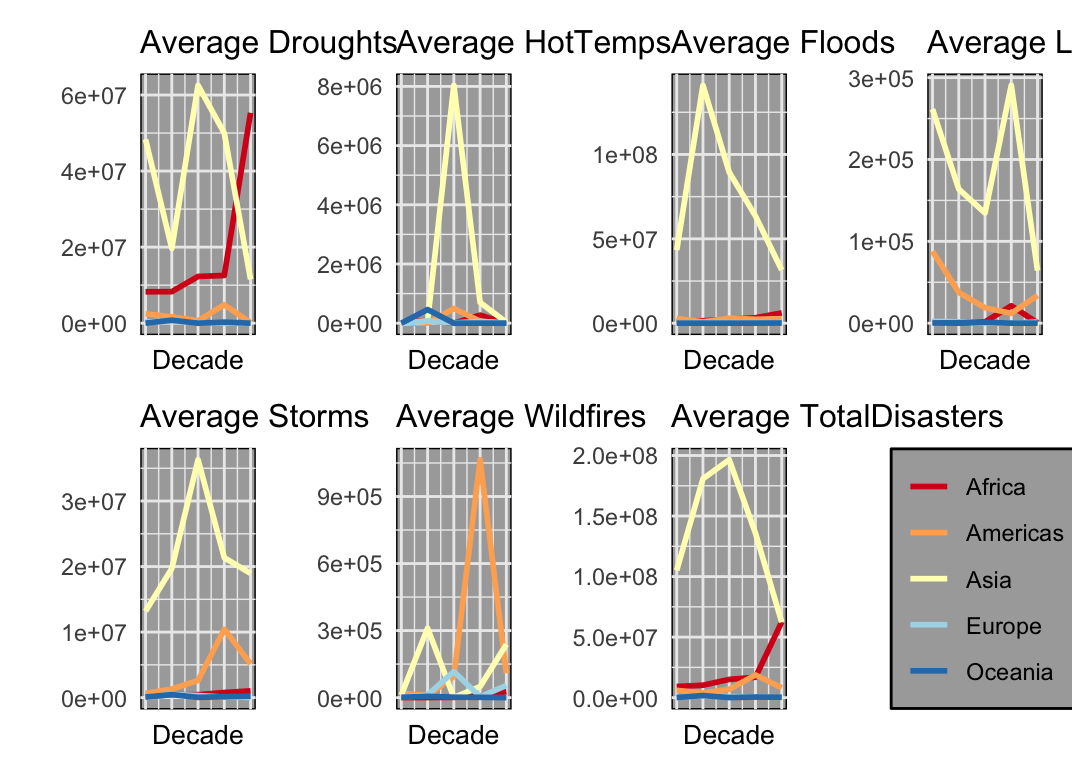
\includegraphics[width=5.5cm]{images/disaster/Average_disaster.png}
	\end{center}
\end{frame}

\subsection{}
\begin{frame}
	\frametitle{Remarks on Climate Related Disasters}
	\begin{itemize}
	\item Asia appears to have the most disasters both on average and in total. 
        \item The only place that had a worse category is in the Americas for wildfires. 
        \item However, it appears that Africa surpassed them in droughts. 
    \end{itemize}
\end{frame}

%%%%%%%%%%%%%%%%%%%%%%%%%
\section{Sea Level Changes}  
%%%%%%%%%%%%%%%%%%%%%%%%%


\subsection{}
\begin{frame}
	\frametitle{Sea Level Changes} % Posture 8
	\begin{center} 
		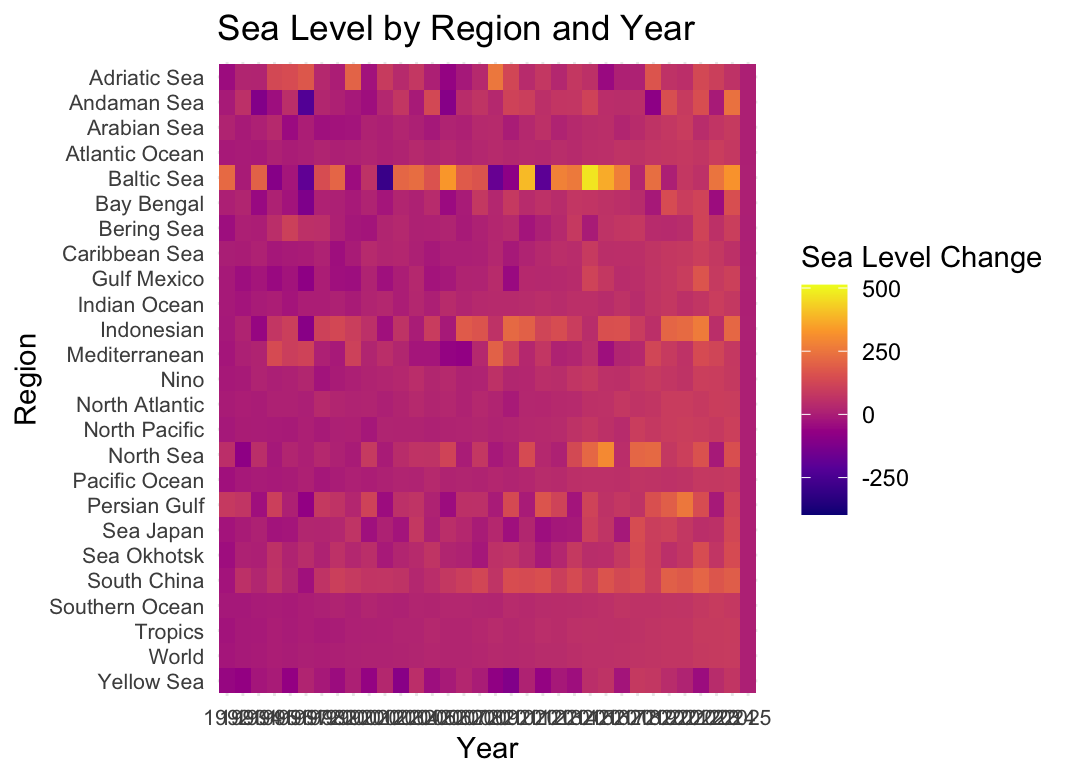
\includegraphics[width=5.5cm]{images/sea_level_heatmap.png} \hspace{1pt}
		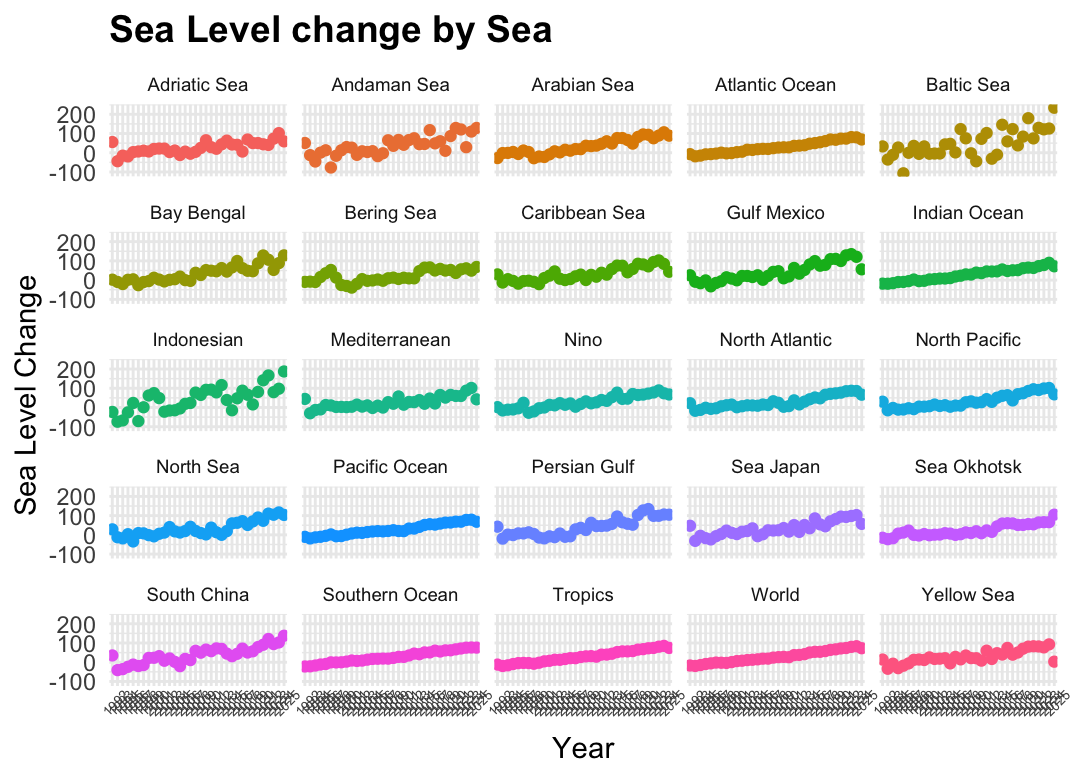
\includegraphics[width=5.5cm]{images/Sea_level_plot.png}
	\end{center}
\end{frame}

\subsection{}
\begin{frame}
	\frametitle{Remarks on Sea Level Changes}
	\begin{itemize}
	\item It appears to have gotten warmer in every ocean and sea in the world. \\[1cm]
        \item There appears a steady incline in all areas. 
    \end{itemize}
\end{frame}

%%%%%%%%%%%%%%%%%%%%%%%%%
\section{Forest and Carbon Levels}  
%%%%%%%%%%%%%%%%%%%%%%%%%

\begin{frame}
	\frametitle{Comparative map of Log Forest Area around the World} % Posture 14
	\begin{center} 
		\animategraphics[loop,autoplay,width=0.7\linewidth]{10}{images/gif_frames/frame_}{000}{064} \hspace{1pt}
	\end{center}
\end{frame}

\subsection{}
\begin{frame}
	\frametitle{Remarks on Forest Area}
	\begin{itemize}
	\item There appears to be less log forest area now then there was in the 1990s\\[1cm]
        \item This might cause some of the issues with temperature and disasters
    \end{itemize}
\end{frame}

%%%%%%%%%%%%%%%%%%%%%%%%%
\section{Conclusions and Outlook}  
%%%%%%%%%%%%%%%%%%%%%%%%%

\begin{frame}
	\frametitle{Conculsions} 
	\begin{itemize}
	\item As the temperature as increased across the globe, other aspects of the climate has been impacted.
        \begin{itemize}
            \item Disasters have fluctuated but do appear to be more common in current years
            \item All sea levels have appeared to have risen
            \item Log Forest Area appears to have decreased across the globe. 
            \item The forest might be the only one to not be an "effect" and rather a cause of the temperature rising
        \end{itemize}
	\end{itemize}
\end{frame}


\begin{frame}
	\frametitle{Future Analysis} 
	\begin{itemize}
	\item Things that we would like to investigate in the future:
	\begin{itemize}
	    \item Which is the cause of the relationship between the forest area and rising temperatures?
        \item How many people are affected by the growing number of disasters?
        \item Have disasters become more destructive recently compared to the past?
        \item Are there other indicators from other sources that we should be worried about?
	\end{itemize}
	\end{itemize}
\end{frame}

% References: Syrjala, 4 test aggregations, Chunyang R package; Syrjala applications for eye tracking

\begin{frame}
	\frametitle{References and Resources} 
	\scriptsize
	\begin{itemize}
	\item Call of the Data Analysis 
    \begin{itemize}
        \item \url{https://iasc-isi.org/2025/01/14/call-of-the-data-analysis-competition-2025/}
    \end{itemize}
        \item Climate and Weather Dashboard (Surface Temperature Change, Mean Sea Level Changes)
        \begin{itemize}
            \item \url{https://climatedata.imf.org/pages/climate-and-weather}
        \end{itemize}
        \item Mitigation Dashboard (Forest and Carbon)
        \begin{itemize}
        \item \url{https://climatedata.imf.org/pages/mitigation}
        \end{itemize}
        \item Adaptation Dashboard (Climate Related Disasters)
        \begin{itemize}
            \item \url{https://climatedata.imf.org/pages/mitigation}
        \end{itemize}
	\end{itemize}
\end{frame}


\subsection{}
\begin{frame}
	\frametitle{}
	\begin{itemize}
	\item {\large \bf Questions ?!?} \\[1cm]
    \end{itemize}
\end{frame}



\end{document}